\documentclass{article}


\usepackage[italian]{babel}
\usepackage{listings}
\usepackage{color}
\usepackage{colortbl}

\definecolor{dkgreen}{rgb}{0,0.6,0}
\definecolor{gray}{rgb}{0.5,0.5,0.5}
\definecolor{mauve}{rgb}{0.58,0,0.82}

\lstset{frame=tb,
  language=Bash,
  aboveskip=3mm,
  belowskip=3mm,
  showstringspaces=false,
  columns=flexible,
  basicstyle={\small\ttfamily},
  numbers=none,
  numberstyle=\tiny\color{gray},
  keywordstyle=\color{blue},
  commentstyle=\color{dkgreen},
  stringstyle=\color{mauve},
  breaklines=true,
  breakatwhitespace=true,
  tabsize=3
}

\usepackage[letterpaper,top=2cm,bottom=2cm,left=3cm,right=3cm,marginparwidth=1.75cm]{geometry}

% Useful packages
\usepackage{amsmath}
\usepackage{graphicx}
\usepackage[colorlinks=true, allcolors=blue]{hyperref}

\title{{\fontsize{31}{30}\sffamily\textbf{Relazione Progetto di \\ Algoritmi e Strutture Dati}}
	\author{
	\large\textbf{Apollonio Francesco:} 0000971247
		    \vspace{1em}\\
	\large\textbf{Frau Alessandro:} 0000971546
	    \vspace{4em}\\
		
\includegraphics[width=74mm]{UniBo-Universita-di-Bologna.png}\vspace{4em}\\
		Progetto ASD A.A. 2021-2022\\
		Corso di Laurea in Informatica \\
		Dipartimento di Informatica - Scienza e Ingegneria \\
		Università di Bologna}
        %\vspace{3.5em}\\
		%Geophysical Institute, \\
		%University of Bergen
	%}
	\huge\date{\today}
}


\begin{document}

\maketitle

\newpage
\tableofcontents
\newpage

\section{Introduzione}
\subsection{(M, N, K)-Game}
Trattasi di una versione avanzata del classico gioco del Tris.
In particolare, (M, N, K)-Game è un gioco in cui due giocatori, a turni, si alternano andando a marcare, ognuno con un simbolo differente, una cella vuota di una griglia di dimensioni (M x N).
L'obiettivo di ogni giocatore è quello di marcare, col proprio simbolo, una serie di (K) celle \textbf{consecutive}. Tali celle possono essere allineate in orizzontale, verticale oppure in diagonale.
Il primo giocatore che riesce nell'obiettivo vince la partita; se nessuno dei due ci riesce e terminano le celle vuote nella griglia allora il risultato finale sarà un pareggio per entrambi.

\subsection{Il Progetto}
Il progetto richiede lo sviluppo di un Player software in grado di giocare, in maniera quanto più intelligente possibile, a tutte le istanze possibili di un ( M, N, K )-Game.
E' ovvio che, per ottenere un'intelligenza artificiale di questo genere, siano necessari algoritmi più o meno complessi computazionalmente. 
E' dunque obiettivo implicito del progetto quello di ottenere un bilanciamento tra efficenza e intelligenza del Player; segue un'approfondita anlisi delle scelte implementative effettuate con tali finalità.

\section{Scelte implementative}
\subsection{Eval}
Tra le scelte implementative di maggior rilevanza abbiamo sicuramente quella dell'Eval.
La valutazione ottimale di una situazione di gioco può, infatti, fare la differenza in un progetto in cui il costo computazionale è oggetto di particolare attenzione. Segue il funzionamento concettuale del nostro Eval.
\medskip

Data una matrice di gioco (M,N,K) generiamo rispettivamente:
\begin{itemize}
\item Una matrice di dimensioni (M, \textit{M-K+1}) per tenere traccia dei simboli allineati orizzontalmente
\item Una matrice di dimensioni (\textit{N-K+1, N}) per tenere traccia dei simboli allineati verticalmente
\item Due matrici di dimensioni (\textit{M-K+1}, \textit{N-K+1}) per tenere traccia dei simboli allineati in diagonali: una matrice per i simboli che vanno dal basso verso l'alto e l'altra per i simboli dall'alto verso il basso.
\end{itemize}

Ognuna delle matrici generate rappresenta virtualmente uno spazio all'interno della matrice di gioco in cui è possibile completare una serie di K simboli consecutivi. 
In questo modo terremo traccia di ogni spazio della board in cui sia possibile raggiungere una vittoria.

\newpage

\textbf{ESEMPIO}

\medskip
Data una semplice istanza di gioco (3,3,3) genereremo le seguenti matrici:
\begin{itemize}
\item Una matrice colonna di altezza 3.
\item Una matrice riga di lunghezza 3.
\item Due matrici 1x1.
\end{itemize}

Le 4 matrici che generiamo dispongono, inoltre, di una terza dimensione; essa è costante ed è 2. La prima delle due dimensioni serve per poter salvare la situazione di gioco valutando \underline{esclusivamente} i simboli inseriti dal nostro player. La seconda dimensione conterrà dunque la situazione di gioco valutando \underline{esclusivamente} i simboli inseriti dal player avversario.
\medskip

Vediamo ora graficamente l'esempio appena introdotto.

\begin{figure}[!h]
\centering
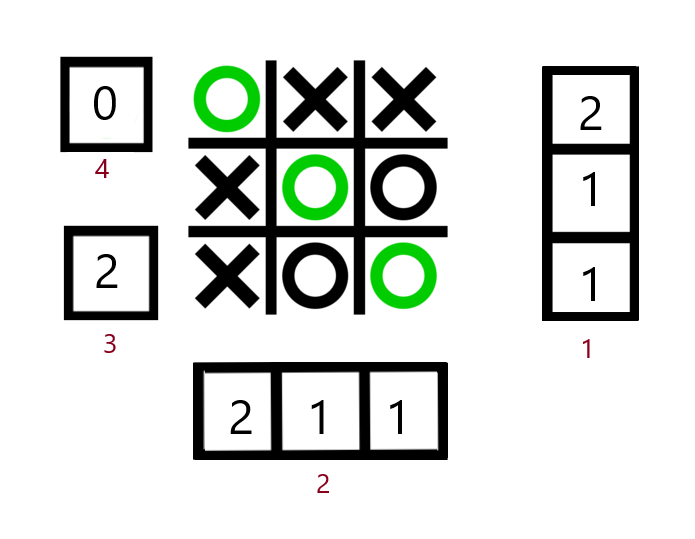
\includegraphics[width=0.5\columnwidth]{MatriciEvalNostre.png}
\caption{Matrici dell'Eval per il nostro Player (Simbolo X)}
\end{figure}

In questo caso notiamo come, ad esempio, nella matrice colonna numero 1 abbiamo rispettivamente: 2 in corrispondenza della prima riga, in quanto su di essa vi sono 2 simboli X, ed 1 in corrispondenza della riga centrale, in quanto su di essa vi è un solo simbolo X. Il ragionamento è poi analogo per la restante cella e la matrice numero 2.

Per quanto riguarda la matrice numero 3 essa contiene il numero di simboli X contenuti nella diagonale che va dal basso a sinistra in alto a destra.
La matrice numero 4, analogamente, contiene il numero di simboli X presenti nella diagonale che va dall'alto a sinistra in basso a destra.

\newpage

\begin{figure}[!h]
\centering
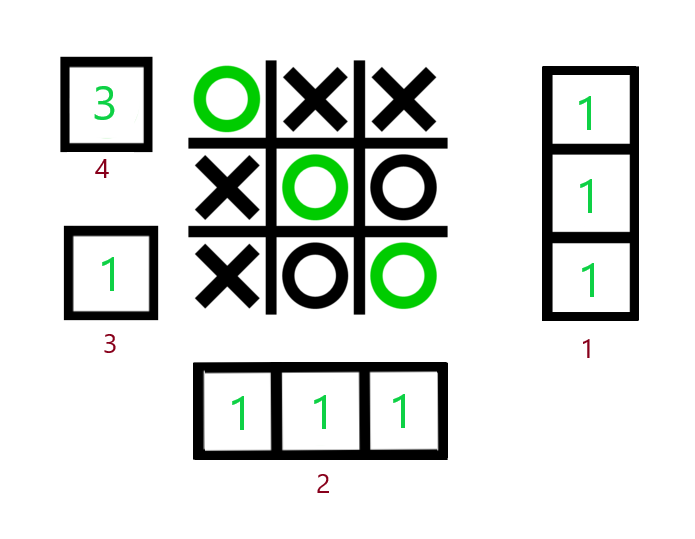
\includegraphics[width=0.5\columnwidth]{MatriciEvalAvversario.png}
\caption{Matrici dell'Eval per il Player avversario (Simbolo O)}
\end{figure}

Il ragionamento per cui sono riempite le celle è analogo a quello illustrato sopra.
Notiamo che in questo caso la matrice numero 4 ha valore 3 == K ( In quanto ricordiamo di star giocando in una configurazione 3,3,3 ) e restituirà quindi una vittoria per l'avversario.

\medskip

Valutando opportunamente le matrici generate il nostro Eval è quindi in grando di assumere uno dei seguenti stati
\begin{itemize}
\item \textbf{WIN}: La board ha una vittoria assicurata.
\item \textbf{CANT LOSE}: Il player avversario non può vincere.
\item \textbf{DRAW}: Pareggio ASSICURATO.
\item \textbf{NOT DEFINED}: Non è stata ancora trovata una valutazione finale.
\item \textbf{CANT WIN}: Il nostro player non può vincere in alcun modo.
\item \textbf{LOSE}: Il nostro player ha una sconfitta assicurata.
\end{itemize}
\medskip
Gli stati sono descritti in ordine di preferenza: in gioco, quindi, si sceglierà di seguire una strada etichettata come "WIN" ad una "CANT WIN", oppure un "DRAW" ad un "LOSE".
\newline
\newline
\textbf{N.B.} "DRAW" e "NOT DEFINED" sono considerati allo stesso livello; nel caso DRAW il pareggio è assicurato, dunque, non esiste assolutamente modo di perdere o vincere qualsiasi siano le mosse successive.
\newline
\newline
Ogni stato è, inoltre, accompagnato da uno score; questo serve per poter decidere quale situazione è più conveniente per noi a parità di stato.

Lo score è assegnato come segue:
\begin{itemize}
    \item Nel caso degli stati definitivi (WIN, LOSE e DRAW), lo score rappresenta la profondità alla quale quello stato viene rilevato. Dunque, ad esempio, se troviamo una DRAW con score 8, sappiamo che a quella profondità raggiungiamo uno stato di DRAW con assoluta certezza.
    \begin{itemize}
        \item Nel caso di DRAW e LOSE lo score viene massimizzato, in questo modo cerchiamo di perdere o pareggiare il piu tardi possibile.
        \item Nel caso della WIN lo score viene invece minimizzato.
    \end{itemize}
    \item Nel caso degli stati non definitivi (NOT\_DEFINED, CANT\_WIN e CANT\_LOSE), lo score corrisponde a quello dell'eval, dunque viene sempre massimizzato.
\end{itemize}


\subsection{Perchè questo Eval?}
Tra i tanti vantaggi ottenuti dall'utilizzo di un Eval come questo spiccano sicuramente: 
\begin{itemize}
\item Capacità di determinare una situazione di pareggio con largo anticipo.
\item Ridotto costo computazionale dell'aggiornamento delle matrici generate.
\end{itemize}

In primo luogo, infatti, ci rendiamo conto di come possa risultare immediato rilevare la presenza di un pareggio con largo anticipo; per ogni cella delle matrici dell'eval generate è, infatti, sufficiente che sia presente almeno un simbolo di entrambi i player per determinare un pareggio assicurato in quello specifico spazio.
Se tutte le 4 matrici dell'Eval genereranno poi un pareggio quello sarà il miglior risultato finale della partita in corso.

\medskip

Per quanto riguarda il costo computazionale, dato che teniamo traccia delle mosse precedenti, ogni valutazione di una mossa consisterà nello scorrere all'interno delle matrici dell'eval, per un massimo di $(k-1)$ celle, in ognuna delle 4 direzioni in modo da aggiornarne i valori considerando la nuova mossa. \newline 
Ogni aggiornamento avrà, dunque, nel caso peggiore, un costo di $4 * (K - 1)$ che ammortizzato risulterà essere $O(K)$. \newline
C'è anche da considerare la fase di annullamento delle mosse che costerà quanto la fase di aggiornamento, portando ad un costo finale di $2 * O(K)$ che ammortizzato sarà ancora $O(K)$.\newline
\newline
Possiamo, inoltre, facilmente notare quanto sia efficiente l'aggiornamento di ognuna di queste matrici (dell'Eval) per ogni turno. Esse infatti vengono aggiornate con costo quasi costante \textit{O(K)}
necessitando della somma di un numero, al risultato parziale, per ogni aggiornamento.

\subsection{AlphaBeta}
Alla base del nostro Player abbiamo inoltre l'utilizzo di un algoritmo di \textit{AlphaBeta-Pruning} con \textit{Negamax}; l'\textit{AlphaBeta-Pruning} è un algoritmo di ricerca utilizzato per ridurre drasticamente il numero di nodi esplorati e valutati dall'algoritmo \textit{Negamax}.
Questo tipo di algoritmo è utile perché tramite il taglio di alcuni sottoalberi del nostro \textit{gametree} riesce a permettere l'esplorazione dell'albero di gioco in profondita' molto piu elevate. Abbiamo, inoltre, preferito utilizzare l'algoritmo \textit{Negamax} invece del \textit{Minimax} per una questione stilistica del codice ed, in particolare, abbiamo scelto di utilizzare la variante \textit{Fail Soft} dell'algoritmo: riteniamo sia più ottimale tagliare il maggior numero di nodi possibile.

\subsection{Iterative Deepening}
Utilizziamo anche una strategia di iterative deepening. Essa è una strategia di attraversamento del Game tree che permette di gestire al meglio il tempo e l'attraversamento dell'albero stesso. E' stato inoltre dimostrato che, nonostante le ripetizioni di nodi attraversati, tramite l'ordinamento e altre tecniche utilizzate permette di attraversare l'albero in maniera piu rapida. Nel pratico, tale strategia consiste nell'attraversare l'albero mettendo un'altezza limite che parte da 1, e cresce ogni volta che l'altezza precedente è stata completata. Grazie all'iterative deepening siamo in grado di proseguire la nostra ricerca fino allo scadere del tempo fornito, e non abbiamo la necessità di fermarci dopo un numero prefissato di nodi esplorati per evitare di andare in timeout.
\subsection{Transposition Table}
Una \textit{Transposition Table} è un database che salva i risultati delle ricerche precedentemente effettuate, in modo da ridurre al minimo il numero di volte che viene ripetuta una ricerca identica. Questo database è estremamente utile perché, durante una partita, capita molto spesso che si arrivi a ricercare il valore di due board identiche, presenti in due rami diversi del game tree. Dunque, utilizzando le transposition table siamo in grado di evitare ricerche ridondanti rendendo così il nostro algoritmo più efficiente.

Il funzionamento generale è comunque abbastanza intuitivo, infatti la \textit{Transposition Table} non è altro che una hash table, in cui vengono salvati: 
\begin{itemize}
\item long hash: Per verificare che il valore nella transposition table sia lo stesso che stiamo cercando.
\item CustomScore   eval:       Lo score trovato.
\item BitSet        type:       Il tipo di score salvato.
\item int           depth:      La profondita' in cui è stato trovato lo score.
\item int           maxDepth:   La profondita' massima di ricerca quando è stato trovato lo score.
\item MNKCell       next:       La migliore mossa successiva a questa.
\end{itemize}
La tabella accetta $2^{23}$ entry, quindi non è ad indirizzamento diretto in quanto ogni hash ha una dimensione di 64 bit ($2^{64}$ possibili hash, contro le $2^{23}$ entry massime della tabella), dunque per l'indirizzamento viene fatto \textit{hash modulo numero di entry}, e questo causa collisioni di indice.
\subsubsection{Collisioni di indice}
Per evitare di assegnare a due posizioni diverse lo stesso valore, solo perché hanno lo stesso indice nella tabella, all'interno di ogni entry viene salvato anche l'hash completo, da confrontare prima di assegnare il valore alla posizione corrente. Per gestire le collisioni utilizziamo una gestione \textit{Always Replace}, infatti ogni volta che troviamo un valore da inserire nella tabella, lo inseriamo, a prescindere che ci sia gia' un valore presente in quell'indice o meno. Abbiamo scelto questo approccio perché, nonostante il fatto che il costo computazionale di questo approccio è nullo (dato che non effettuiamo nessun controllo), la probabilita' che il valore nuovo sia piu importante di quello gia inserito nella tabella è abbastanza alta, perché spesso due board identiche raggiunte da percorsi differenti, sono abbastanza vicine anche nell'albero. 

\subsubsection{Hashing}
Come algoritmo di hashing utilizziamo quello di Zobrist.\newline
\textit{Zobrist Hashing} è una tecnica di hashing che trasforma lo stato di una board di dimensione arbitraria in un valore di lunghezza prefissata, con una distribuzione equa rispetto a tutti i possibili valori ottenibili. All'inizio dell'esecuzione viene generato un array di valori pseudorandomici, uno per ogni simbolo moltiplicato per ogni posizione nella tabella (per esempio in un 3x3, abbiamo 2 simboli, X e O, e 9 posizioni, dunque genera 18 valori randomici). Per ottenere il valore della board corrente, viene effettuato lo xor tra tutti i valori corrispondenti alle mosse effettuate dai giocatori per arrivare allo stato che si sta valutando. \newline

\subsubsection{Collisione di Hash}
Una \textit{Key Collision} avviene quando due board distinte vengono codificate nello stesso hash. Queste collisioni sono inevitabili, ma possono essere ridotte al minimo variando la dimensione della tabella.


\subsubsection{Ricerca tabelle simmetriche}
Un altra ricerca che abbiamo effettuato nelle transposition table è quella delle board simmetriche; ogni board può, infatti, essere ruotata e, nonostante gli hash risultanti siano diversi il loro stato è identico. In particolare: nei casi di board rettangolari effettuiamo una rotazione di 180 gradi e nei casi di board quadrate effettuiamo tre rotazioni di 90 gradi. Analogamente, specchiamo la board corrente ed effettuiamo ancora tutte le rotazioni dette in precedenza. Quindi, per ogni board valutata, nel caso sia rettangolare otteniamo al più 4 valutazioni della stessa, mentre nel caso sia quadrata ne otteniamo massimo 8.


\subsection{Move ordering}
Un'altra tecnica che abbiamo utilizzato per migliorare il nostro player è quella di ordinare le mosse prima di proseguire nel Game tree. Abbiamo creato una classe che si occupa dell'ordinamento, e in questa classe abbiamo utilizzato un algoritmo di \textit{Quicksort} con costo computazionale di $O(n\cdot log(n))$ dove $n$ è il numero di celle libere. L'algoritmo è stato scritto da noi per poter utilizzare i confronti custom degli score. Aggiungere questo algoritmo al nostro player ha un costo computazionale variabile a seconda della profondità fino a cui vogliamo effettuare l'ordinamento, dunque varierà da player a player.

\section{Testing and Benchmarking}

\subsection{Per linee generali}
Per poter avere un riscontro pratico di ogni miglioramento portato dall'aggiunta di ogni features, abbiamo deciso di creare un Player differente per ogni step.
Seguono i differenti Player sviluppati:
\begin{enumerate}
    \item PlayerNegamax: risultante applicando esclusivamente gli algoritmi di NegaMax ed Eval.
    \item PlayerBetterNegamax: risultante modificando il modo di incrementare lo score (che adesso avviene in fattori di 10).
    \item PlayerAlphaBeta: risultante dall'applicazione dell'algoritmo di AlphaBeta al Player precedente.
    \item PlayerMoveOrder: risultante applicando la tecnica di Move Ordering al player Alphabeta solo al primo livello di profondità.
    \item PlayerSecondLayerMoveOrder: risultante applicando la tecnica di Move Ordering al player Alphabeta, solo per i primi due livelli di profondità.
    \item PlayerFullMoveOrder: risultante applicando la tecnica di Move Ordering al player Alphabeta ad ogni livello di profondità.
    \item PlayerTransposition: risultato dell'applicazione delle Transposition Table al player AlphaBeta.
    \item PlayerCutsTransposition: risultato della modifica dell'applicazione delle Transposition Table al player precedente, aggiungendo i tagli anche per score non esatti ma solo riferiti a lowerbound e upperbound.
\end{enumerate}
In questo modo, sfidando i Player fra di loro, ci rendiamo concretamente conto dei miglioramenti portati da ogni step. Analizziamo nelle sezioni successive i risultati ottenuti. 
In particolare abbiamo fatto sfidare tra loro solo i player migliori ottenuti dopo ogni cambiamento sostanziale.

\subsection{Tool utilizzati}
Per poter far sfidare i Player tra di loro, e quindi analizzarne i risultati, abbiamo sviluppato uno script in linguaggio Bash: \textit{benchmark.sh}

Tale script permette di automatizzare la compilazione e la sfida dei differenti Player in diverse serie di tabelle di gioco predefinite. 
Per ottenere dei risultati analizzabili abbiamo scriptato le sfide usando le istanze di gioco note (quindi con risultato finale conosciuto) forniteci dall'insegnante. 

Per ogni Board in cui avviene la sfida i due Player giocheranno un totale di 4 partite.
Nelle prime due uno dei Player avrà la prima mossa, nelle seconde due la prima scelta toccherà invece all'altro giocatore.
Ogni partita vinta assegnerà 3 punti al vincitore, ogni patta 1 ad entrambi.
Alla fine di ogni partita verrà visualizzato il risultato finale.

Durante lo svolgimento di ogni partità verranno salvate tutte le mosse scelte, nonchè diversi dati ( profondità raggiunta, tagli effettuati ecc. ), in un file di log. 



Abbiamo inoltre implementato dei file in python:
\begin{itemize}
    \item \textit{benchmark\_parser.py}: utilizzato per ottenere lo score finale (quindi la somma di tutti gli score) di un file di log.
    \item \textit{recap\_benchmark.py}: utilizzato per leggere gli score per ogni round da un file di log.
    \item \textit{round\_recap.py}: utilizzato dallo script \textit{benchmark.sh}, da non eseguire su un file di log.
\end{itemize}

\textbf{N.B.} Affinchè lo strumento di benchmark descritto funzioni è necessario utilizzare i pacchetti MNK-Game da noi modificati.

\newpage

\subsection{Benchmarking}
In questa sezione analiziamo i risultati ottenuti dalla sfida tra i diversi nostri Player.
\subsubsection{Sfide interne}
Come prima cosa, per ogni player che implementano le stesse features (se pur con piccole modifiche), avvengono delle sfide per decretare quale delle minori modifiche implementate è la migliore.
\begin{itemize}
    \item \textbf{Negamax}: Nel negamax abbiamo fatto sfidare i player Negamax e BetterNegamax, per capire se effettivamente la modifica ha portato ad un miglioramento.
    \begin{itemize}
        \item PlayerNegamax - PlayerBetterNegamax: 89 / 98 \textbf{PlayerBetterNegamax} vince.
    \end{itemize}
    
    
    \item \textbf{Transposition Table}: Nelle transposition table abbiamo fatto sfidare i player Transposition e CutsTransposition, per verificare che l'aggiunta dei tagli porti ad un miglioramento. 
    \begin{itemize}
        \item PlayerTransposition - PlayerCutsTransposition: 95/96 \textbf{PlayerCutsTransposition} vince.
    \end{itemize}
    
    
    \item \textbf{Move Order}: Nel move order abbiamo fatto sfidare MoveOrder, FullMoveOrder e SecondLayerMoveOrder, per vedere quale delle alternative fosse la migliore nell'ordinamento.
        \begin{itemize}
            \item PlayerSecondLayerMoveOrder - PlayerFullMoveOrder: 97/111 \textbf{PlayerFullMoveOrder} vince 
            \item PlayerMoveOrder - PlayerFullMoveOrder: 144/64, \textbf{PlayerMoveOrder} vince.
            \item PlayerMoveOrder - PlayerSecondLayerMoveOrder: 131/73, \textbf{PlayerMoveOrder} vince.
        \end{itemize}
         Quindi il migliore di questa categoria è \textbf{PlayerMoveOrder}
\end{itemize}
\subsubsection{Sfide finali}
In questa sezione analizziamo le sfide tra i migliori Player di ogni categoria: il vincitore sarà il nostro miglior Player.
\begin{center}
    \begin{table}[htpb]
    \centering
        \begin{tabular}{||c | c | c | c ||}
             \hline
                & CutsTransposition & Alphabeta & MoveOrder \\
             \hline\hline
             BetterNegamax & \cellcolor{yellow}98-98 &\cellcolor{red} 83-110 &\cellcolor{red} 95-99 \\
             \hline
        \end{tabular}
    \end{table}
\end{center}
\begin{center}
    \begin{table}[htpb]
    \centering
        \begin{tabular}{||c | c | c | c ||}
             \hline
                & BetterNegamax & Alphabeta & MoveOrder \\
             \hline\hline
             CutsTransposition & \cellcolor{yellow}98-98 &\cellcolor{red} 86-107 &\cellcolor{red} 76-118 \\
             \hline
        \end{tabular}
    \end{table}
\end{center}
\begin{center}
    \begin{table}[htpb]
    \centering
        \begin{tabular}{||c | c | c | c ||}
             \hline
                & BetterNegamax & CutsTransposition & MoveOrder \\
             \hline\hline
             Alphabeta & \cellcolor{green} 110-83 &\cellcolor{green} 107-86 &\cellcolor{red} 74-123 \\
             \hline
        \end{tabular}
    \end{table}
\end{center}
\begin{center}
    \begin{table}[htpb]
    \centering
        \begin{tabular}{||c | c | c | c ||}
             \hline
                & BetterNegamax & CutsTransposition & Alphabeta \\
             \hline\hline
             MoveOrder & \cellcolor{green}99-95 &\cellcolor{green} 118-76 &\cellcolor{green} 123-74 \\
             \hline
        \end{tabular}
    \end{table}
\end{center}
\newpage
Dunque abbiamo trovato che il player più forte è \textbf{PlayerMoveOrder}
\section{Osservazioni}
\subsection{Spiegazione dei risultati non identici su configurazioni uguali}
Alcuni risultati possono non essere identici su due partite uguali per due motivi: l'ordine con cui sono state proposte le mosse è diverso oppure la CPU ha lavorato meglio in una delle due partite ed è riuscita, dunque, ad analizzare più mosse. Aldilà di questo il codice, eccetto quello delle transposition table, è deterministico e, quindi, a parità di nodi esplorati e di ordine iniziale delle mosse, porterà allo stesso risultato.
\subsection{Alphabeta è piu forte di Transposition}
A seguito dei vari benchmark, ma anche durante la fase di implementazione, ci siamo accorti che anche dopo aver implementato le transposition table, Alphabeta risultava più forte. Dunque, nel tentativo di dare una risposta a questo, abbiamo sviluppato varie teorie e conclusioni che elenchiamo di seguito.
\subsubsection{Bug}
La prima cosa a cui viene da pensare è sicuramente la presenza di qualche bug nel codice; è ovvio che non sia possibile affermare con assoluta certezza che non ce ne siano, ma, a seguito della revisione di tutti i logfile riguardanti le partite di Alphabeta contro Transposition Table, possiamo evincere che il problema non sia legato a bug evidenti nelle aggiunte implementative, bensì ad altri fattori di cui discutiamo in seguito.

\subsubsection{L'implementazione non vale quello che costa}
Confrontando i logfile ci siamo resi conto di come il numero di nodi esplorati dal semplice Alphabeta fosse nettamente maggiore del numero di nodi esplorati dalla Transposition Table. Ma maggiore di quanto? Ovviamente questo dipende dal calcolatore, ma possiamo dire che Transposition Table esplorava circa 1/5 dei nodi che riusciva ad esplorare Alphabeta. Da qui possiamo concludere che probabilmente, nonostante in proporzione il numero dei tagli fosse maggiore  il costo dell'implementazione non vale il miglioramento che porta.

\section{Utilizzo del codice}

\subsection{Locazione dei file utili}
I differenti Player sviluppati possono essere trovati all'interno della cartella "BottargaPlayer".
Qui troviamo una serie di sottocartelle: una per ognuno di essi.
All'interno di ciascuna di esse vi sono i file utilizzati per sviluppare esclusivamente il Player in questione; tra questi il file rappresentante il Player pronto a giocare, quindi quello che implementa \textit{MNKPlayer} è quello nominato "\textit{Player.java}". Il resto dei file, che sono all'interno di "\textit{Utils}", fanno da scheletro alle nostre configurazioni e contengono tutto il codice utilizzato in comune dai nostri player.


\subsection{Compilazione ed esecuzione}

Locarsi nella cartella \textit{MNKGame2.0}.
\medskip
Da qui lanciare il seguente comando per compilare:

\begin{lstlisting}
javac -d source BottargaPlayer/*/*.java mnkgame/*.java
\end{lstlisting}
\medskip
Ed il seguente comando per eseguire una sfida tra i Player sviluppati:

\begin{lstlisting}
java mnkgame.MNKPlayerTester M N K BottargaPlayer.PlayerDirectory.Player BottargaPlayer.PlayerDirectory.Player -v -t 10 -r 1
\end{lstlisting}
Dove M N K va sostituito con la configurazione con la quale si vuole eseguire la sfida e 'PlayerDirectory' va sostituito con la cartella all'interno della quale è presente il Player che si vuole far giocare.

\subsection{Main del player finale}
Ricordiamo inoltre che il player che vogliamo far giocare nella competizione tra colleghi è il piu forte tra quelli che abbiamo implementato: \textbf{BottargaPlayer.PlayerMoveOrder.Player}

\section{Idee future}
Abbiamo avuto altre idee in corso di sviluppo, ma per motivi di tempo non siamo riusciti ad implementarle, dunque ci limitiamo a citarle qui:
\begin{itemize}
    \item Precalcolo dei dati: un'idea molto interessante era quella di calcolare in anticipo le mosse da eseguire, salvando solo quelle più rilevanti in un file testuale. 
    Questo metodo sembra interessante in quanto permette anche con pochissime risorse (infatti si potrebbero salvare anche solo le prime due o tre mosse che peserebbero pochi byte in memoria) di instradare il giocatore verso una giocata molto spesso migliore di quella che può calcolare nei soli 10 secondi concessi. Sarebbe una tecnica paragonabile al seguire tattiche di apertura del gioco negli scacchi.
    
    \item Controllo di K-1: Un'altra tecnica che quasi certamente avrebbe portato un miglioramento nel nostro player è quella di osservare, nelle matrici dell'Eval, tutte le celle che hanno valore uguale a K-1; infatti queste celle, se non bloccate nella mossa corrente, portano ad una sconfitta certa, e dunque hanno come conseguenza una mossa ovvia. Utilizzare questa tecnica porterebbe all'aumento del livello di quiescenza di uno, e dunque migliorerebbe quasi certamente il nostro player, visto e considerato anche che con l'implementazione attuale dell'eval fare questo tipo di controllo avrebbe costo costante.
\end{itemize}

\end{document}
